\documentclass[10pt]{article}
\usepackage[utf8]{inputenc}
\usepackage{cite}
\usepackage{graphicx}
\usepackage{amsmath}
\usepackage{listings}
\usepackage{kbordermatrix}
\usepackage{subcaption}
\graphicspath{ {../results/2017-01-06/} }

\title{Predicting signal peptides}
\author{Simon Karlsson \\ sikar@kth.se}
\date{\today}

\begin{document}
\maketitle

\begin{abstract}
Many proteins needs help by the signal peptide with relocation to the actual location in the cell where the protein is to perform its task.
The signal peptide is not present in all proteins, which raises he question of how one can determine if the signal peptide is part of a given protein or not.
This project examines two different machine learning methods, the naïve Bayes classifier and the support vector machine classifier, from the scikit-learn Python library, to distinguish signal peptides from non-signal peptides.
The proteomes are represented as a tf-idf matrix and training and testing is done with the Python library scikit-learn against two test sets with two different organisms.
Naïve Bayes performs best with 64\% and 63\% accuracy on the two different test sets.
The accuracy of SVM was 62\% and 60\% on the corresponding test sets.
\end{abstract}

\newpage

\section{Introduction}
A protein is a molecule with extensive responsibility, constructed by chains of amino acids.
The responsibilities of different proteins includes protecting the body from virus and bacteria, carry out chemical reactions in cells and more\cite{website:ghr}.
Many proteins needs help with relocation to the actual location in the cell where they are to perform their task.
This relocation is done by a part of the protein, a molecular unit called signal peptide.
However, not all proteins contains the signal peptide\cite{website:project-description}, which raises the question of how one can determine if the signal peptide is part of a given protein or not.

One historical approach to determine this is with experimental data\cite{website:project-description}, but this is not possible if there is lack of such data.

This project examines two different machine learning methods, the naïve Bayes (NB) classifier and the support vector machine (SVM) classifier, from the scikit-learn Python library, to distinguish signal peptides from non-signal peptides.

\subsection{Structure of this report}
Chapter 2 will go through the materials used and the methods for obtaining the results of this project.
Chapter 3 will present the results and discuss them.
Furthermore, it will present improvements which could improve the results of the project.

\section{Methods and Materials}

\subsection{Data}
The proteomes are represented as strings with each amino acid as one of the characters R, H, K, D, E, S, T, N, Q, C, U, G, P, A, V, I, L, M, F, Y, W.
\subsubsection{Training data}
The data used for training can be found here \cite{website:project-description}.
It consists of 2654 samples, separated into 1320 positive samples (containing signal peptides) and 1334 negative
samples (not containing signal peptides), and is shown in Table \ref{table:trainingdata}.

\begin{table}[h]
\begin{center}
\begin{tabular}{| l | l | l | l |}
\hline
Positive & Negative & Total\\ \hline
1320 & 1332 & 2652\\ \hline
\end{tabular}
\end{center}
\caption{Summary of the traning data used}
\label{table:trainingdata}
\end{table}

\subsubsection{Test data}
The test data was downloaded from Ensembl's BioMart service \cite{website:ensembl}
and consists of samples from two organisms; Red junglefowl (Gallus Gallus) and Rat (Rnor). The number of samples
after preprocessing is shown in Table \ref{table:testdata}.

\begin{table}[h]
\begin{center}
\begin{tabular}{| l | l | l | l |}
\hline
Organism & Positive & Negative & Total\\ \hline
Gallus Gallus & 3435 & 3435 & 6870\\ \hline
Rnor & 4354 & 4354 & 8708\\ \hline
\end{tabular}
\end{center}
\caption{Summary of the test data used}
\label{table:testdata}
\end{table}

\subsection{Training}
The sequences were transformed into a tf-idf representation. This was done with the scikit-learn modules CountVectorizer and TfidfTransformer.
CountVectroizer was used to count the number of occurrences of each amino acid over all training samples. This results in a matrix C of amino acid counts.
The columns represent amino acids and the rows sequences.
The example in matrix \ref{eq:C} contains five sequences (s1 to s5) containing a total of five amino acids (a1 to a5). Sequence 4 consists of 6 amino acids of type 1, 11 of type 2 and so on.

This representation was then transformed into a tf-idf representation using TfidfTransformer. It converts each entry in the matrix to a normalized value between 0 and 1 which is a weighted value of how many times a amino acid appears in a sequence and how important each amino acid is, given how many times it appears in other sequences.
An example of a tf-idf matrix is shown in matrix \ref{eq:M}.

\renewcommand{\kbldelim}{(}
\renewcommand{\kbrdelim}{)}
\[
  \text{C} = \kbordermatrix{
    & a_1 & a_2 & a_3 & a_4 & a_5 \\        s_1 & 47 & 2 & 38 & 15 & 45 \\        s_2 & 5 & 2 & 1 & 5 & 1 \\        s_3 & 1 & 1 & 4 & 1 & 2 \\        s_4 & 6 & 11 & 2 & 10 & 11 \\        s_5 & 2 & 1 & 9 & 9 & 14
  }
\]
\begin{equation}
\label{eq:C}
\end{equation}
\[
  \text{M} = \kbordermatrix{
    & a_1 & a_2 & a_3 & a_4 & a_5 \\        s_1 & 0.17 & 0.08 & 0.33 & 0.08 & 0.08 \\        s_2 & 0.06 & 0.37 & 0.21 & 0.36 & 0.21 \\        s_3 & 0.36 & 0.21 & 0.23 & 0.17 & 0.26 \\        s_4 & 0.15 & 0.42 & 0.30 & 0.34 & 0.08 \\        s_5 & 0.12 & 0.32 & 0.11 & 0.19 & 0.20
  }
\]
\begin{equation}
\label{eq:M}
\end{equation}
The target labels is put in a vector where the index corresponds to the row index of the tf-idf matrix. The vector in figure \ref{eq:t} shows an example where sequence 1-3 contains signal peptides and 4-5 do not contains signal peptides.
\[
  \text{t} = \kbordermatrix{
    & t_1 & t_2 & t_3 & t_4 & t_5 \\        & 1 & 1 & 1 & 0 & 0 \\
  }
\]
\begin{equation}
\label{eq:t}
\end{equation}

The tf-idf matrix and the target vectors are input to the MultinomialNB and SVC functions from the python library scikit-learn as in figure \ref{eq:commands} below.

\begin{lstlisting}
    MultinomialNB().fit(tfidf, targets)
    SVC(kernel="rbf").fit(tfidf, targets)
\end{lstlisting}
\begin{equation}
\label{eq:commands}
\end{equation}

\subsection{Testing}
At testing, the sequences were converted to a tfidf-vector exactly as in training, that is, based on how many times a amino acid appears in a sequence and how important each amino acid is, given how many times it appears in other sequences in the training set.
When predicting multiple sequences, this yields a matrix like matrix \ref{eq:M} above.
To predict if each sequence contained a signal peptide the scikit-learn function predict was used on the classifier obtained by the training, which is shown in figure \ref{eq:predict} below.

\begin{lstlisting}
classifier.predict(tfidf)
\end{lstlisting}
\begin{equation}
\label{eq:predict}
\end{equation}

This method returns a list of zeros and ones, each one corresponding to a sequence in the testing, where 1 means that the sequence is predicted to contain a signal peptide and 0 means that the sequence is predicted to not contain a signal peptide.

\subsection{Controls}
During this project some controls were used to establish that the software was working as expected and that the results were not just based on random noise.

The program was executed with completely random data for training and testing of the models. For both the NB and SVM model, this resulted in a correct guess 50 \% of the times as expected with completely random data. This indicates that the results are significant and not just based on noise.

Too short sequences were discarded and sequences containing more letters than existing amino acids were also discarded.

General error checking with associated error messages was implemented for I/O operations with the strategy to always abort when an error occurred, so that no partial results were created.

\section{Results and Discussion}
Table \ref{table:rnorresults} summarizes the result on the Rnor test data set, and
table \ref{table:gallusresults} summarizes the result on the Gallus Gallus data set.
Figure \ref{fig:results} displays the results for both data sets in a bar chart.

\begin{table}[h]
\begin{center}
\begin{tabular}{| l | l | l | l | l |}
\hline
Method & Positive & Negative & Total\\ \hline
Bayes & 0.6672026 & 0.6129995 & 0.6401011\\ \hline
SVM & 0.6109325 & 0.6208085 & 0.6158705\\ \hline
\end{tabular}
\end{center}
\caption{Results for Rnor}
\label{table:rnorresults}
\end{table}
\begin{table}[h]
\begin{center}
\begin{tabular}{| l | l | l | l | l |}
\hline
Method & Positive & Negative & Total\\ \hline
Bayes & 0.5988355 & 0.6532751 & 0.6260553\\ \hline
SVM & 0.5397380 & 0.6561863 & 0.5979621\\ \hline
\end{tabular}
\end{center}
\caption{Results for Gallus Gallus}
\label{table:gallusresults}
\end{table}
\begin{figure}[p]
\begin{subfigure}{\textwidth}
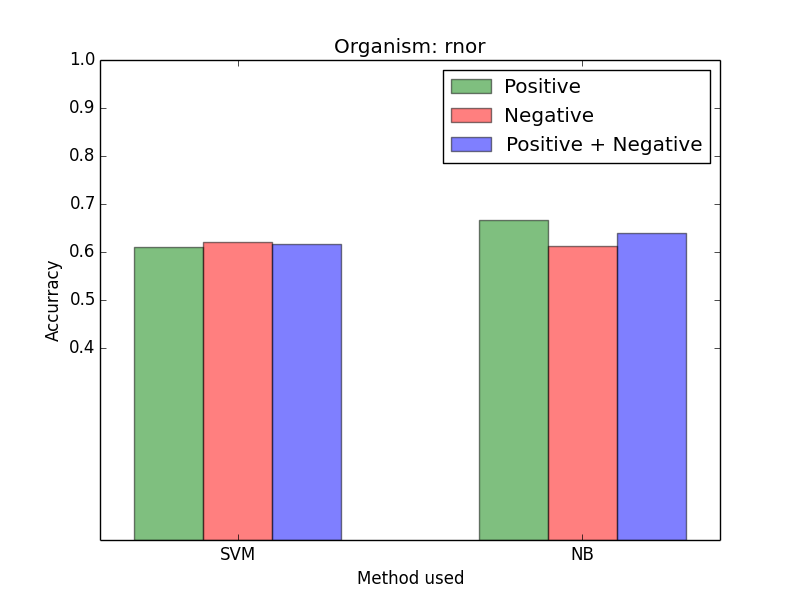
\includegraphics[width=1.0\linewidth]{rnor}
\caption{Results for Rnor}
\label{fig:rnor}
\end{subfigure}
\begin{subfigure}{\textwidth}
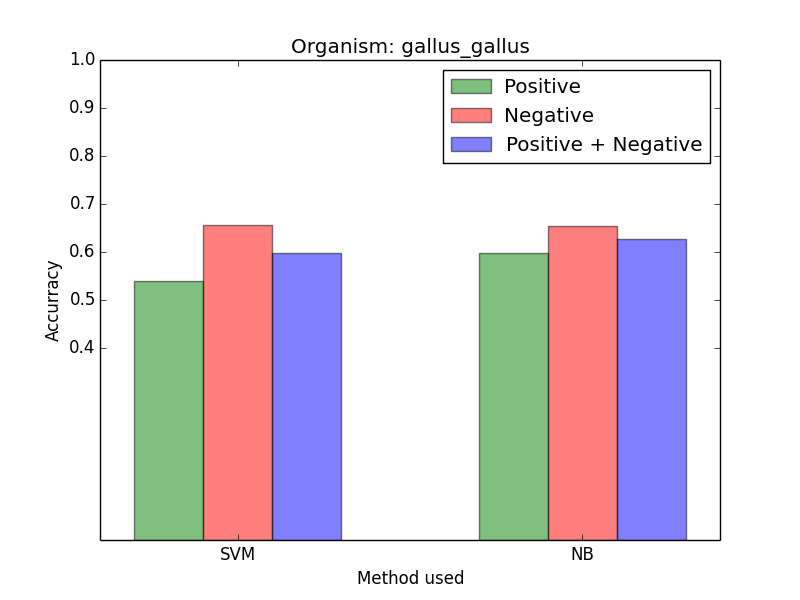
\includegraphics[width=1.0\linewidth]{gallus_gallus}
\caption{Results for Gallus Gallus}
\label{fig:gallus}
\end{subfigure}
\caption{Results}
\label{fig:results}
\end{figure}

The NB classifier performs better than the SVM classifier on both test sets when considering both positive and negative samples.

The SVM performs better on both test sets considering only the negative samples, this is however compensated for due to the substantial better performance for the NB classifier on the positive samples for both test sets.

All in all, an accuracy somewhere between 59\% and 65\% can be expected when predicting signal peptides with NB and SVM with the python library scikit-learn using the default setting without any parameter optimization.
Performing better than mere chance this shows that it is possible to predict signal peptides with a machine learning approach.
However, the basic method used in this report results in an accurracy that is probably to low to be useful in a practical setting.

\subsection{Future improvements}
With some improvements to the method used in this project, predicting signal peptides with machine learning could be made useful for a practical setting.
\subsubsection{Parameter fitting}
The methods used for this project are very crude, with all the parameters set to default
by scikit-learn with only some parameter optimization on the class weights for the SVM classifier
based on manual testing. The result could be improved by some proper parameter fitting using
cross validation.
\subsubsection{Consider transmembrane sequences}
One known issue with predicting signal peptide is that part of the signal peptides could look lika a transmembrane region, which means that a transmembrane structure could be mistaken for a signal peptide\cite{website:project-description}.
This issue could be taken in consideration somehow when predicting signal peptides to improve the result.
\subsubsection{More data}
The results could possible be improved if the models were trained with more data.
\subsubsection{Other methods}
It would also be relevant to test more methods than just Naïve Bayes and SVM.

\subsection{Implementation of Stafford Noble's ideas}
The work process of this project was based on the ideas of William Stafford  Noble \cite{stafford}. This sections discusses these ideas.
\subsubsection{Files and Directory Organization}
The organization of files and directories was created exactly as recommended by
Staffor Noble with the folders src, data, results and doc at the root. The data was placed
under a directory stating the date when the data was downloaded. Links to the data
was dynamically generated given the date when the data was downloaded. All the results were also
under a directory stating which date the results were generated.
\subsubsection{Lab notebook}
A lab notebook was used during the project. I have never work in this fashion
with a notebook so in the beginning I often forgot to document my progress and the
notes tended to be quite sparse throughout the project. However, towards the end of
the project my note became better, and I can see that there is much to gain by tending
a notebook, when you need to go back and see what you did earlier on in the project.
\subsubsection{Carrying out a single experiment}
Stafford Noble stated that it was good to save all command lines used to produce
the result. Since my commands were very simple I found that i did not need to do this.
However, with more complicated commands I can see the point of doing that. I saved all
paths used during the experiments in a Constants file where the paths were generated dynamically
based on the date identifier on the data folders, so that the program
will work independently of the structure of the operating system.
\subsubsection{Handling and Preventing Erros}
General error with associated error messages were implemented for I/O operations.
I took the approach suggested by Stafford Noble to abort on errors, trying to avoid
creating partial results.
\subsubsection{Version Control}
Github was used for this project. Stafford Noble mentions three reasons for using
version control; backup, possibility to do rollbacks and collaboration. Since I did
this project alone the collaboration part was not important to me. However, having
backups and the possibility to do rollbacks is important for all software projects.

\bibliography{ref}{}
\bibliographystyle{plain}

\end{document}
